In this section we describe how we have performed the testing of our system.
We have basically followed the guidelines already defined in our Design document so, if you want additional information, please refer to sections 6.4 and 6.5 of that document.
As regards ApplicationServer subsystem, since in the DD we have described the testing strategy of the entire planned subsystem, we do not have performed the testing of the entire system but only until event EventManager integration (please refer to our design document to see the order of integration).\\
\begin{figure}[H]
	\begin{center}
		\hspace*{-40pt}
		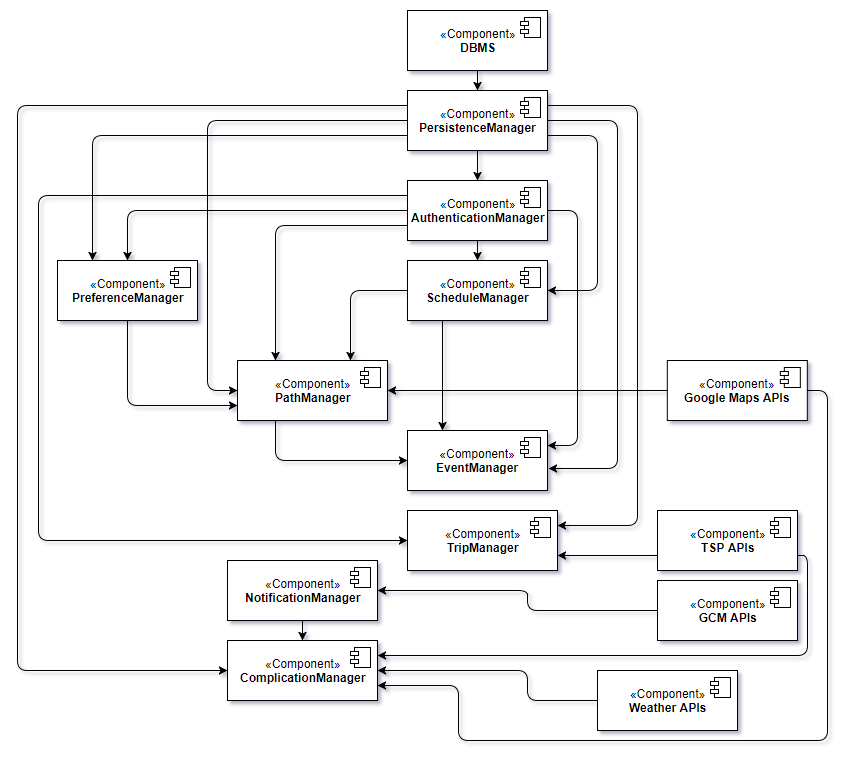
\includegraphics[scale=0.4]{app_server_I&T.png}
	\end{center}
\caption{ ApplicationServer - Actually tested subsystems subsystems}
\end{figure}
For what concerns the Android App subsystem we have tested the DAOs that interact with the local DB. \\
These tests can be found in test/java/it/polimi/travlendarplus, as can be seen in the previous chapter "Source code structure". \\
To run these tests it is enough to right click on them in Android Studio and select "Run".

\section{Procedure Adopted}
\subsection{Persistence manager (JPA - DBMS interaction): Arquillian}
In order to perform our \textit{PersistenceManager}'s testing we have adopted the following procedure: we have exploited Arquillian features to obtain a testing configuration that allow us to use a testing container of GlassFish that can run and connect to an embedded GlassFish 3.1 instance.
Our \textit{PersistenceManager}'s tests simply  persist a set of sample entities to the database, connected with the GlassFish container, and then retrieve them using JPA Criteria API.
Each test method checks that the sample data retrieved from the database is correct. Before and after a test is performed, the database is cleaned up, in order to guarantee that each test is run in a clean environment.
This is the outcome of these tests:
\begin{figure}[H]
	\begin{center}
		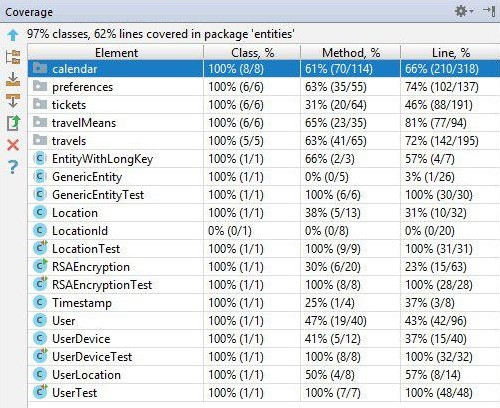
\includegraphics[scale=0.7]{JPA_test_outcome.jpg}
	\end{center}
\caption{ \textit{PersistenceManager} - code coverage}
\end{figure}

\subsection{Enterprise Java Beans: Mockito}
We used Mockito to test the \textit{PathManager}, a Stateless EJB that requires other Stateless EJBs (\textit{ScheduleManager} and \textit{PreferenceManager}) in order to perform its tasks. Making use of Mockito, all the functions performed by one of the injected beans were mocked: the idea is to consider these functions as working and to test the instructions properly defined in the \textit{PathManager}.\\\\
In particular, we mocked \textit{ScheduleManager} functions in this way:
\begin{itemize}
\item for each function that returns an event a predefined event is returned, depending on the parameter passed to the function;
\item for \textit{PathCalculation} function a random response is returned, based on the travels passed to the function;
\item for save functions a \textit{doNothing} method is used.
\end{itemize}  
\textit{PreferenceManager} functions are mocked in this way:
\begin{itemize}
\item \textit{checkConstraints} function return always \textit{true};
\item \textit{findBestPath} function return always the first element in the array of possibilities.\\
\end{itemize}
We tested \textit{calculatePath} function, a function that for a given event returns previous and following paths according to the other events in the schedule. We considered a general case in which both previous and following events exist and the cases in which one of them doesn't exist; we verified that:
\begin{itemize}
\item the previous path is between the end of the previous event and the start of the current event;
\item the following path is between the end of the current event and the start of the following event;
\item the starting location of the previous path is the location of previous event or a location specified by the user;
\item the ending location of the previous path is the location of the current event;
\item the starting location of the following path is the location of current event or a location specified by the user;
\item the ending location of the following path is the location of the following event.
\end{itemize}
We tested also \textit{swapEvents} function, a function that forces an overlapping event into the schedule and removes from the schedule all the events in conflict with the added one. We verified the right behavior of the function in these cases:
\begin{itemize}
\item base case with the swap out of an overlapping event;
\item swap out of a previous event no more feasible due to the path calculation of the added event;
\item swap out of a following event no more feasible due to the path calculation of the added event;
\item swap in feasible with an overlapping but feasible break event;
\item swap in feasible after the swap out of a no more feasible break event.\\
\end{itemize}
We used Junit in order to test the beans that don't contain components difficult to test.
\begin{figure}[H]
	\begin{center}
		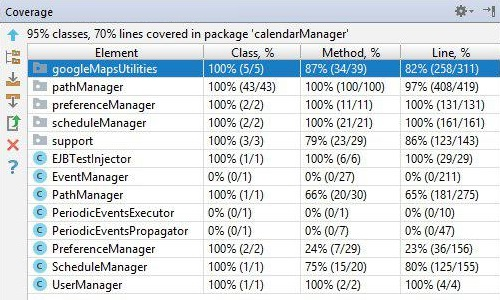
\includegraphics[scale=0.7]{CalendarManager_test_outcome.jpg}
	\end{center}
\caption{ \textit{CalendarManager} - code coverage}
\end{figure}

\subsection{RESTful API: JMeter}


